%\pdfoutput=1

\documentclass{article}
\usepackage{authblk}
\usepackage{todonotes}
\usepackage[margin=1in]{geometry}
\usepackage[parfill]{parskip}
\usepackage{times}
\usepackage{graphicx}
\usepackage{caption}
\usepackage{subcaption}
\usepackage{tikz}
\usepackage{pgfplots}
%\usepackage{natbib}
\usepackage{float}
\usepackage{algorithm,algpseudocode}
\usepackage{rotating}
%\usepackage{algorithmic}
\usepackage{amsfonts,amsmath,amsthm,amssymb}
\usepackage{mathtools}
\usepackage{hyperref}
\newcommand{\theHalgorithm}{\arabic{algorithm}}
\usepackage[shortcuts]{extdash}
\newcommand{\SREC}{S\=/REC}
\DeclareMathOperator*{\argmin}{arg\,min}
\DeclareMathOperator*{\argmax}{arg\,max}
\def\R{{\mathbb{R}}}
%\newtheorem{theorem}{Theorem}[section]
\newcommand{\mb}[1]{\mathbf{#1}}
\newtheoremstyle{exampstyle}
  {10pt} % Space above
  {10pt} % Space below
  {} % Body font
  {} % Indent amount
  {\bfseries} % Theorem head font
  {.} % Punctuation after theorem head
  {.5em} % Space after theorem head
  {} % Theorem head spec (can be left empty, meaning `normal')
\theoremstyle{exampstyle} \newtheorem{theorem}{Theorem}[section]

\newtheorem{corollary}{Corollary}[theorem]
\newtheorem{lemma}[theorem]{Lemma}
\newtheorem{definition}{Definition}
%\title{Compressed Sensing on GANs using Iterative Projections}
\title{Reconstruction from Modulo Measurements}
\date{}
\def\sgn{\mathrm{sgn}}
\def\t{\intercal}
\def\cosamp{\mathrm{CoSaMP}}
\author{Viraj Shah}
\author{Chinmay Hegde}
\affil{ECpE Department, Iowa State University}

\newcommand{\norm}[1]{\|#1\|}
\newcommand{\eps}{\epsilon}
\newcommand{\wh}[1]{\widehat{#1}}
\newcommand{\s}{0.18}
\usepackage{hyperref}
\usepackage[utf8]{inputenc}
\usepackage{booktabs}
\usetikzlibrary{calc}
\begin{document}
\vspace{-25em}
\maketitle
\input{./model}
\section{Mathematical Analysis}
\label{sec:mathanalysis}

Before presenting experimental validation of our proposed MoRAM algorithm, we now perform a theoretical analysis of both the initialization and the descent stages, and provide an upper bound on the number of samples required for accurate sparse signal recovery under the Gaussian observation model.

\subsection{Analysis of the initialization}
Recall that we perform the initialization in two steps:
(i) measurement correction step, and (ii) estimation step. We analyze them separately.

\subsubsection{Measurement correction step}\label{meascorr} In this step, based on the magnitude of the modulo measurements, we identify the measurements for which we can undo the effect of modulo transfer function by guessing the correct value of bin-index $\mathbf{p}$. We define the set $U$ as set of indices of all such measurements that can be corrected. We determine the measurements to be corrected based on the method described in section~\ref{sec:init}. 

In this analysis, our goal is to estimate the number of measurements ($N=\card(U)$) that can be corrected. Only these $N$ measurements would be used in the estimation step. Each element of $\mb{A}$ is chosen i.i.d. from a standard normal distribution. Therefore, $\mu_{\mb{A}_{ij}} = 0$ and $\sigma_{\mb{A}_{ij}}=1$. 

Recall that:
$$
y_{c,i} =\langle \mathbf{a_i} \cdot \mathbf{x^*} \rangle = \sum_{j=1}^{n}\mb{A}_{ij}x^*_{j}.
$$
Being a linear combination of Gaussian random variables, the corrected observations $y_{c,i}$ also follows Gaussian distribution:
$$
\mu_{y_{c}} = \sum_{j=1}^{n}x^{*}\mu_{\mb{A}_{ij}} = 0,
$$
$$
\sigma_{y_{c}} =\sum_{j=1}^{n}x^{*2}_{j} \sigma^2_{\mb{A}_{ij}} = \sum_{j=1}^{n}x^{*2}_{j} = \norm{\mathbf{{x}^*}}^2 = 1;
$$
$$
\implies y_{c,i} \sim \mathcal{N}\left(\mu= 0, \sigma = 1 \right)
$$
Hence, each element of $\mathbf{y_c}$ follows a zero mean Gaussian distribution with unit variance.

We can calculate $N$ using the fact that the compressive measurements $y_c$ follow the standard normal distribution, and the total number of measurements are $m$. We define $\mathcal{M}_{\alpha,\beta}$ as the set of all measurements lying in the interval $[\alpha,\beta]$. Thus,

Here, $\card\left(\mathcal{M}_{\alpha,\beta}\right)=mP(\alpha \leq y_{c,i}\leq \beta) = m\left(Q(\alpha)- Q(\beta)\right)$
where, $Q(\cdot)$ is the Gaussian Q-function defined as:
$$Q(t) = 1-\Phi(t)$$ 
with $\Phi(\cdot)$ being the CDF of standard normal distribution. We also note that:
 $$Q(-t) = 1 - Q(t).$$
The Q-function does not have a closed form expression. However, it can be bounded by the following functions where $\phi(\cdot)$ is standard normal density function:
$$
\left(\frac{t}{1+t^2}\right)\phi(t) < Q(t) < \frac{\phi(t)}{t}.
$$
Therefore, for $R > \rho$,
\begin{align}
N & = \card\left(\mathcal{M}_{-R + \rho,0}\right) + \card\left(\mathcal{M}_{0, R-\rho}\right) \nonumber \\
N &  = m\left(Q(-R+\rho)- Q(0)\right) + m\left(Q(0)- Q(R-\rho)\right) \nonumber \\
& = m\left(Q(-(R-\rho))- Q(R-\rho)\right) \nonumber \\
& = m\left(1-2Q(R-\rho)\right). \nonumber
\end{align}
Using the bounds above,
\begin{align}
N \geq m \left(1-2\frac{\phi(R-\rho)}{(R-\rho)} \right).
\label{eq:n_bound}
\end{align}
%\noindent case (ii). $R < \rho$: In this case,
%\begin{align}
%N & = \card\left(\mathcal{M}_{-\rho,-R}\right) + \card\left(\mathcal{M}_{R,\rho}\right) \nonumber \\
%N & = m\left(Q(-\rho)- Q(-R)\right) + m\left(Q(R)- Q(\rho)\right) \nonumber \\
%& = m\left(1 - Q(\rho)-1 +Q(R) +Q(R) -Q(\rho)\right) \nonumber \\
%& = 2m\left(Q(R)-Q(\rho)\right).
%\end{align}
%
%Using the bounds above,
%$$
%N \geq 2m \left(\frac{R}{(1+R^2)} \phi(R) - \frac{\phi(\rho)}{\rho}\right).
%$$
For a given \emph{total} number of observed measurements $m$, Eq.~\ref{eq:n_bound} provides the lower bound on the value of $N$, the number of \emph{correctable} measurements.

\subsubsection{Estimation step}
Using the corrected measurements (denoted as set $U$), we can compute an initial estimate of the signal using a simple first-order thresholded estimator:
$$
\mathbf{{x}^0} = H_s\left(\frac{1}{\card(U)}\sum_{i\in U}y_{i}a_{i}\right).
$$
$$
\mb{x^0} = H_s\left( \frac{1}{N}\sum_{i=1}^{N}y_{U,i}a_{U,i}\right)
$$
where $H_s(\cdot)$ denotes the hard thresholding operator (that retains the $s$-largest magnitude coefficients of a given vector.  We use the versions of $\mb{y}$ and $\mb{A}$ truncated to the row indices belonging to set $U$, and column indices to set $S$. We denote such sub-matrices with the subscript $U\times S$. 

We can now prove that our initial estimate as constructed above is close to the true signal $\mb{x^*}$. We obtain:

\theorem{Let $\delta \in (0,1)$ and $t \geq 1$. The initial estimate $\mb{x^0}$ is the output of the algorithm~\ref{alg:RCM}. If the total number of corrected measurements satisfy, $N \geq C(\frac{t}{\kappa})^2s$, where $\kappa = \frac{\delta}{2}$, then  with probability at least $1 - 2\left(\frac{en}{s}\right)^s\exp\left(-t^2s\right)$ we have,
	$$
	\norm{\mb{x^0} - \mb{x^*}}_2 \leq \delta \norm{\mb{x^*}}_2.
	$$
	\label{th:1}
}

\proof {We define $\mb{\tilde{x}^0}$ as the value of the initial estimate before the hard thresholding step:
$$
\mb{\tilde{x}^0} = M = \frac{1}{N}\sum_{i=1}^{N}y_{U,i}a_{U,i} =  \frac{1}{N}\mb{A}_U^\t\mb{y_U}.
$$
Substituting $\mb{y_U}=\mb{A}_U\mb{x^*}$,
$$
\mb{\tilde{x}^0} = M = \frac{1}{N}\mb{A}_U^\t \mb{A}_U\mb{x^*}.
$$

We note that each row of our truncated Gaussian measurement matrix ($\mb{A}_{\scriptscriptstyle{U\times S}}$) is independent, and also follows the Gaussian distribution with zero mean.  
We denote this distribution with Gaussian random vector $Z$ in $\R^s$, and arrange $N$ rows as the independent samples from the distribution; $Z_i := \mb{A}_{\scriptscriptstyle{U\times S},i}$. 
Recall that the covariance matrix of $Z$ can be calculated as $\Sigma = \mathbb{E}Z\otimes Z$,
$$
\Sigma= \mathbb{E}Z\otimes Z = \mathbb{E} ZZ^\t = \diag{\mathbb{E}z_1^2,\mathbb{E}z_2^2,...,\mathbb{E}z_n^2} = I_n.
$$

Now, calculating the sample covariance matrix of $Z$ using the samples $Z_i = \mb{A}_{\scriptscriptstyle{U\times S},i}$,
$$
\Sigma_N = \frac{1}{N}\sum_{i=1}^{N}Z_i \otimes Z_i = \frac{1}{N} \mb{A}_{\scriptscriptstyle{U\times S}}^\t \mb{A}_{\scriptscriptstyle{U\times S}}.
$$

Given $N \geq C\left(\frac{t}{\kappa}\right)^2s$, we invoke Corollary 5.50 of~\cite{vershynin2010introduction} which relates $\Sigma_N$ and $\Sigma$ as follows, with probability at least $1 - 2\exp\left(-t^2s\right)$:

\begin{align*}
\norm{\Sigma_N - \Sigma}_2 &\leq \kappa,~~~~~\text{i.e.,} \\
\norm{\frac{1}{N} \mb{A}_{\scriptscriptstyle{U\times S}}^\t \mb{A}_{\scriptscriptstyle{U\times S}} - I_s}_2 &\leq \kappa \\
\end{align*}

We now use a standard covering number argument. Let us fix the $s$_sparse vector $\mb{x^*}$ within the unit norm ball. We can evaluate the operator norm in above equation over the set of $s-$sparse vectors in the unit norm ball.
\begin{align*}
\implies \sup_{\mb{x} \in S} \frac{\norm{\left(\frac{1}{N} \mb{A}_{\scriptscriptstyle{U\times S}}^\t \mb{A}_{\scriptscriptstyle{U\times S}} - I_n\right)\mb{x}}_2}{\norm{\mb{x}}_2} &\leq \kappa \\
\norm{\left(\frac{1}{N} \mb{A}_{\scriptscriptstyle{U\times S}}^\t \mb{A}_{\scriptscriptstyle{U\times S}} - I_n\right)\mb{x^*}}_2 &\leq \kappa \norm{\mb{x^*}_2} \\
 \norm{\left(\frac{1}{N} \mb{A}_{\scriptscriptstyle{U\times S}}^\t \mb{A}_{\scriptscriptstyle{U\times S}}\mb{x^*} - \mb{x^*}\right)}_2 &\leq \kappa \norm{\mb{x^*}_2} \\
 \norm{\mb{\tilde{x}^0} - \mb{x^*}}_2 &\leq \kappa \norm{\mb{x^*}}_2 
\end{align*}
with probability at least $1 - 2\exp\left(-t^2s\right)$ given the fixed $s-$sparse vector $\mb{x^*}$. Taking an union bound over all $n \choose s$ such $s-$sparse vectors,
\begin{align*}
\mathbb{P}\left(\norm{\mb{\tilde{x}^0} - \mb{x^*}}_2 \leq \kappa \norm{\mb{x^*}}_2\right) & \geq 1 - 2{n \choose s}\exp\left(-t^2s\right) \\ 
& \geq 1 - 2\left(\frac{en}{s}\right)^s\exp\left(-t^2s\right)
\end{align*}

The initial estimate $\mb{x^0}$ is the best $s-$sparse estimate of $\mb{\tilde{x}^0}$. We consider,
\begin{align*}
\norm{\mb{{x}^0} - \mb{x^*}}_2 &=  \norm{\mb{\tilde{x}^0} -\mb{\tilde{x}^0} +\mb{\tilde{x}^0} - \mb{x^*}}_2 \\
& \leq \norm{\mb{{x}^0} -\mb{\tilde{x}^0}}_2 +  \norm{\mb{\tilde{x}^0} - \mb{x^*}}_2 \\
& \leq 2 \norm{\mb{\tilde{x}^0} - \mb{x^*}}_2 \\
& \leq 2 \kappa \norm{\mb{x^*}}_2 = \delta \norm{\mb{x^*}}_2
\end{align*}
with probability at least $1 - 2\left(\frac{en}{s}\right)^s\exp\left(-t^2s\right)$.
Last inequality follows from the fact that $\mb{\tilde{x}^0}$ is closer to $\mb{x^0}$ compared to $\mb{x^*}$, because $\mb{x^0}$ is the best $s-$sparse approximation of $\mb{\tilde{x}^0}$. $\qed$}

\subsection{Analysis of descent}
We perform the Alternative Minimization as described in~\ref{alg:MoRAM}, starting with $\mb{x^0}$ calculated as above. However, for simplicity, we limit our analysis of the convergence to only one iteration of our Alternative Minimization based algorithm. In fact, as proven in our analysis, theoretically only one iteration of JP is required for exact signal recovery. Contrast to that, in practice we observe that our algorithm requires more than one alternative minimization iterations to converge to the optimum solution.

The first step is to obtain the initial estimate for bin-index vector, $\mb{p^0}$ using $\mb{x^0}$.
$$
\mathbf{{p}^{0}} = \frac{\mathbf{1}-\sgn(\langle \mathbf{A} \cdot \mathbf{x^0} \rangle)}{2}.
$$
If we try to undo the effect of modulo operation by adding back $R$ for the affected measurements based on the bin-index vector $\mb{p^0}$, it would introduce the error equaling $R$ corresponding to the incorrect bin-index values in $\mb{p^0}$.
$$
\mathbf{y^0_c} = \langle \mathbf{A}\mathbf{x^{0}} \rangle = \mathbf{y} - \mathbf{p^0}R,
$$

In the following theorem, we claim the guaranteed recovery of the true signal as the corruption in the first set of corrected measurements $\mb{y_c^0}$ can be modeled as sparse vector with sparsity less than or equal to $cm$, with $c$ being a fraction.
For the next lemma, we first introduce the concept of binary $\epsilon$-stable embedding as appeared in~\cite{Jacques2013}. We note that $\mathcal{B}^m$ is a Boolean cube defined as $\mathcal{B}^m := \{-1,1\}^m$; and $S^{n-1}:=\{\mb{x}\in \R^n : \norm{\mb{x}}_2 = 1\}$ is the unit hyper-sphere of dimension $n$.
\definition[Binary $\epsilon$-Stable Embedding]{A mapping $F: \R^n \rightarrow \mathcal{B}^m$ is a binary $\epsilon$-stable embedding (B$\epsilon$SE) of order $s$ for sparse vectors if:
	$$
	d_S(\mb{x,y}) - \epsilon \leq d_H(F\mb{(x)},F\mb{(y)}) \leq d_S(\mb{x,y}) + \epsilon;
	$$
	for all $\mb{x,y} \in S^{n-1}$ with $|supp(x) \cup supp(y)|\leq s$.
}

In our case, let's define the mapping $F: \R^n \rightarrow \mathcal{B}^m$ as:
$$
F(\mb{x}):= \sgn(\mb{Ax});
$$
with $\mb{A} \sim \mathcal{N}^{m \times n}(0,1)$.


\lemma{Let $\mb{A}$ be the matrix generated as $\mb{A} \sim \mathcal{N}^{m \times n}(0,1)$ and $\mb{x^*, x^0} \in \R^n$ are $s-$sparse vectors satisfying $\norm{\mb{x^* - x^0}}_2 \leq \delta\norm{\mb{x^*}}_2$. Let $\eta \in [0,1],~\eps > 0$. Given the number of measurements \\
	$m \geq \frac{2}{\eps^2}\left(s\log{(n)} + 2s\log{\left(\frac{35}{\eps}\right)}+\log{\left(\frac{2}{\eta}\right)}\right)$, following is true with probability exceeding $1 - \eta$:
	
	$$
	d_H(\sgn({\mb{Ax^*}}), \sgn({\mb{Ax^0}})) \leq \frac{\delta}{2} + \eps;
	$$
where $d_H$ is Hamming distance between binary vectors defined as:
$$
d_H(\mb{a,b}) := \frac{1}{n}\sum_{i=1}^{n}a_i \oplus b_i,
$$
for $n-$ dimensional binary vectors $\mb{a,b}$.
\label{lemma1} 
} \\
\proof{ 
Given $m \geq \frac{2}{\eps^2}\left(s\log{(n)} + 2s\log{\left(\frac{35}{\eps}\right)}+\log{\left(\frac{2}{\eta}\right)}\right)$, using Theorem 3 from~\cite{Jacques2013} we conclude that $F(\cdot)$ is a B$\eps$SE for $s$-sparse vectors.
Thus for sparse vectors $\mb{x^*, x^0}$:
\begin{align}
\label{eq:th3}
d_H(F\mb{(x^*)},F\mb{(x^0)}) \leq d_S(\mb{x^*,x^0}) + \eps.
\end{align}

Here, $d_S(\cdot)$ is defined as the natural angle formed by two vectors. Specifically, for $\mb{p,q}$ in unit norm ball,
$$
d_s(\mb{p},\mb{q}) := \frac{1}{\pi}arccos\langle\mb{p},\mb{q}\rangle = \frac{1}{\pi}\theta,
$$
where $\theta$ is the angle between two unit norm vectors $\mb{p}$ and $\mb{q}$.

We note that,
$$
\norm{\mb{p-q}}_2 = 2\sin(\frac{\theta}{2}).
$$
Thus,
\begin{align}
\label{eq:dhds}
2d_s(\mb{p},\mb{q}) \leq \norm{\mb{p - q}}_2 \leq \pi d_s(\mb{p},\mb{q})
\end{align}
Combining eq.~\ref{eq:th3} and eq.~\ref{eq:dhds}, we conclude,

$$
d_H(\sgn({\mb{Ax^*}}), \sgn({\mb{Ax^0}})) \leq \frac{1}{2}\norm{\mb{x^*-x^0}} + \eps.
$$

\begin{align}
\label{eq:hd}
\implies d_H(\sgn({\mb{Ax^*}}), \sgn({\mb{Ax^0}})) \leq \frac{\delta}{2} + \eps.
\qed
\end{align}
}


\theorem{Given an initialization $\mb{x^0}$ satisfying $\norm{\mb{x^* - x^0}}_2 \leq \delta\norm{\mb{x^*}}_2$, for $0 < \delta < 1$, if we have number of (Gaussian) measurements satisfying $s \leq \gamma m/\left(\log\left(n/m\right)+1\right)$, then the estimate after the first iteration $\mb{x^1}$ of Algorithm \ref{alg:MoRAM} is exactly equal to the true signal $\mathbf{x^*}$ with probability at least $1-Kexp(-cm)$, with $K$ and $c$ being numerical constants.
}

\proof{In the estimation step, Algorithm \ref{alg:MoRAM} dubs the problem of recovering the true signal $\mb{x^*}$ from the modulo measurements as the special case of signal recovery from sparsely corrupted compressive measurements. As we discussed in section \ref{sec:modeff}, the presence of modulo operation modify the compressive measurements by adding a constant noise of the value $R$ in fraction of total measurements. However,once we identify correct bin-index for some of the measurements using $\mb{x^0}$, the remaining noise can be modeled as structured (specifically, 'sparse') corruption $\mb{d}$ in the formulation:

$$
\mb{y} = \mb{Ax} + \mb{I_nR(p^0-p^*)} = \mb{Ax} + \mb{d}.
$$  
Here, the $\sl{l}0$-norm of $\mb{d}$ gives us the number of noisy measurements in $\mb{y^0_c}$.
%$$
%\textnormal{the number of noisy measurements in~} \mb{y^0_c} = \norm{\mb{d}}_0
%$$

If the initial bin-index vector $\mb{p^0}$ is close to the true bin-index vector $\mb{p^*}$, then $\norm{\mb{d}}_0$ is small enough with respect to total number of measurements $m$; thus, $\mb{\mb{d}}$ can be treated as sparse corruption. If we model this corruption as a sparse noise, then we can employ JP for a guaranteed recovery of the true signal given (i) sparsity of the noise is a fraction of total number of measurements; (ii) sufficiently large number of measurements are available.  

We compute $\norm{\mb{d}}_0$ as,

$$
\norm{\mb{d}}_0 =  \norm{(\mb{p^*-p^0})R}_0;
$$

expanding further,
\begin{align*}
\norm{\mb{d}}_0  & = \frac{\mathbf{1}-\sgn(\langle \mathbf{A} \cdot \mathbf{x^0} \rangle)}{2} -  \frac{\mathbf{1}-\sgn(\langle \mathbf{A} \cdot \mathbf{x^*} \rangle)}{2} \\
& = \frac{\sgn({\mb{Ax^*}})- \sgn({\mb{Ax^0}})}{2} \\
& = \frac{F\mb{(x^*)} - F\mb{(x^0)}}{2} \\
& = d_H(F\mb{(x^*)}, F\mb{(x^0)}). \\
\textnormal{From eq.~\ref{eq:hd},} \\
& \leq \frac{\delta}{2} + \epsilon = \gamma m.
\end{align*}

Algorithm \ref{alg:MoRAM} is essentially a JP formulation based on basis pursuit as described in \cite{Laska2009}. Exact signal recovery from sparsely corrupted measurements is a well-studied domain with uniform recovery guarantees available in the existing literature. We use the guarantee proved in \cite{li2013compressed} for Gaussian random measurement matrix, which states that one can recover a sparse signal exactly by tractable $\mathit{l1}-$minimization even if a positive fraction of the measurements are arbitrarily corrupted. With $\norm{\mb{d}}_0 \leq \gamma m$, we invoke the Theorem $1.1$ from \cite{li2013compressed} to complete the proof.
$\qed$}

\subsection{Minimum number of measurements required}
In this section, we combine the various inequalities involving number of measurements $m$ from above sections to determine the minimum value of $m$ required for successful recovery of the true signal.

The condition on $N$ comes from theorem \ref{th:1},
\begin{align}
N \geq C\left(\frac{t}{\kappa}\right)^2s.
\label{eq:ineq1}
\end{align}

Also from lemma \ref{lemma1},
\begin{align}
m \geq \frac{2}{\eps^2}\left(s\log{(n)} + 2s\log{\left(\frac{35}{\eps}\right)}+\log{\left(\frac{2}{\eta}\right)}\right).
\label{eq:ineq2}
\end{align}

Now for $R> \rho$, we have following from the analysis in section~\ref{meascorr},
\begin{align}
N \geq m \left(1-2\frac{\phi(R-\rho)}{(R-\rho)} \right).
\label{eq:ineq3}
\end{align}

Combining eqs.~\ref{eq:ineq1},\ref{eq:ineq2} \& \ref{eq:ineq3} we get the minimum number of measurements required as,

\begin{align}
m \geq \max & \Bigg[ C\left(\frac{t}{\kappa}\right)^2s \left(1-2\frac{\phi(R-\rho)}{(R-\rho)} \right)^{-1}, \nonumber \\ 
& \frac{2}{\eps^2}\left(s\log{(n)} + 2s\log{\left(\frac{35}{\eps}\right)}+\log{\left(\frac{2}{\eta}\right)}\right)\Bigg].
\label{eq:ineq4}
\end{align}
For $R=4$ and $\rho =3$, the above inequality approximates to,
\begin{align*}
m \geq \max & \Bigg[ 2C\left(\frac{t}{\kappa}\right)^2s, \nonumber \\ 
& \frac{2}{\eps^2}\left(s\log{(n)} + 2s\log{\left(\frac{35}{\eps}\right)}+\log{\left(\frac{2}{\eta}\right)}\right)\Bigg].
\end{align*}
%Similarly for the case when $R<\rho$ we get,
%\begin{align}
%m \geq \max &  \Bigg[C\left(\frac{t}{\kappa}\right)^2s \left(\frac{2R}{(1+R^2)} \phi(R) - \frac{\phi(\rho)}{\rho}\right)^{-1}, \nonumber \\ 
%& \frac{2}{\eps^2}\left(s\log{(n)} + 2s\log{\left(\frac{35}{\eps}\right)}+\log{\left(\frac{2}{\eta}\right)}\right) \Bigg]
%\label{eq:ineq5}
%\end{align}
%With $R=1$ and $\rho =3$, we can approximate it as,
%\begin{align*}
%m \geq \max &  \Bigg[4C\left(\frac{t}{\kappa}\right)^2s, \nonumber \\ 
%& \frac{2}{\eps^2}\left(s\log{(n)} + 2s\log{\left(\frac{35}{\eps}\right)}+\log{\left(\frac{2}{\eta}\right)}\right) \Bigg]
%\end{align*}
\section{Measurement Model}
We consider the problem of recovery of a signal from its modulo measurements obtained through compressive sensing. Simply put, we aim to recover $\mathbf{x^*}\in \R^n$ from the modulo measurements $y_i=\mod(\langle \mathbf{a_i} \cdot \mathbf{x^*} \rangle,R)$ for $i = \{1,2,...,m\}$, where $\mod$ is modulo operation with respect to $R$. Typically, $m<n$. For simplicity, we assume that the modulo function operates only within two periods, one on the either side of the origin, as shown in the Fig.~\ref{fig:graph}. We construct $\mathbf{A} = \left[\mathbf{a_1~a_2~...~a_m}\right]^T$ with i.i.d. Gaussian entries. The primary assumption in our model is that the natural signal $\mathbf{x^*}$ is $s-$sparse in a chosen basis. 

\begin{figure}[h]
	\begin{center}
\begin{tikzpicture}
\draw[<->] (-4,0) -- (4,0) node[right] {$t$};
\draw[->] (0,-1) -- (0,4) node[above] {$f(t)$};
\draw[scale=0.5, dashed, thick] (0,4)--(7,4) node[right]{$R$};
\draw (1.5,-0.5) node(below) {$p_i = 0$};
\draw (-1.5,-0.5) node(below) {$p_i = 1$};
\draw (0,-1.5) node(right) {$f(t) = \mod(t,R)$};
\draw[scale=0.5,domain=-7:0,smooth,variable=\x,cyan, ultra thick] plot ({\x},{\x+4});
\draw[scale=0.5,domain=0:7,smooth,variable=\x,cyan, ultra thick]  plot ({\x},{\x});
\end{tikzpicture}
\end{center}
\caption{\emph{Modified modulo function for the given problem}}
\label{fig:graph}
\end{figure}

We can write the modified equation for the modulo operation under consideration as:
$$
f(t) = \mod(t,R) = t+\left( \frac{1-\sgn(t)}{2}\right)R,
$$
where $\sgn(t)$ is a signum function.

For the measurement model of the given problem, 
We define the corrected linear measurements as: 

$$
y_{c,i} =\langle \mathbf{a_i} \cdot \mathbf{x^*} \rangle.
$$

We also define the bin-index $p^*_i$ as,
$$
p^*_i = \frac{1-\sgn(\langle \mathbf{a_i} \cdot \mathbf{x^*} \rangle)}{2}.
$$
Thus,
$$
y_i = \langle \mathbf{a_i} \cdot \mathbf{x^*} \rangle + p^*_iR = y_{c,i}+p^*_iR.
$$

It is evident that if we can recover $\mathbf{p^*}$ successfully, we can calculate the correct compressed measurements $\langle \mathbf{a_i} \cdot \mathbf{x^*} \rangle$ and use them to reconstruct $\mathbf{x^*}$ with any sparse recovery algorithm such as CoSaMP.


\section{Reconstruction Algorithm}

In this section, we describe our AltMin based approach to recover $\mathbf{x^*}$ and $\mathbf{p^*}$, given $\mathbf{y, A}, s, R$. We call our algorithm MoRAM - Modulo Reconstruction using Alternative Minimization. Our approach comprises of two steps: (i) estimate initialization step, and (ii) Descent step through alternative minimization.

\subsection{Initialization}
\label{sec:init}
Similar to many non-convex techniques, MoRAM also requires an initial estimate $\mathbf{{x}^0}$ that is close to the true signal $\mathbf{{x}^*}$. The basic idea is to calculate the significant indices (or the support of $\mathbf{{x}^*}$, $S=support(\mathbf{{x}^*})$) using the suitable biased estimators, and then calculate the initial estimate using a first order biased estimator $M$ only for those significant indices contained in the support of $\mathbf{{x}^*}$. This initialization procedure is quite simple, and requires the tuning of only one parameter, the sparsity ($s$).

For support estimation, we use measurements $y_{i}$ to construct a biased estimator $L$, for which the marginal $L_{jj}$ corresponding to the $j^{th}$ element is given by:
$$
L_{jj} = \frac{1}{m}\sum_{i=1}^{m}y_{i}^2 a_{ij}^2,~~~\textnormal{for}~~~~j \in {1,...,n}.
$$
Note that the expectation $\mathbb{E}[\mathbf{L}]$ is given by,
$$
\mathbb{E}[L_{jj}] = 4x_{j}^{*2}+2R^2(1-c_1)-2R\norm{\mathbf{{x}^*}}c_2~~~~~\textnormal{where,}~c_1,c_2 \in \mathbb{R}
$$
indicating that a clear separation exists for values of expectation for $j \in S$ and $j \in S^c$, because $x_j$ is zero for $j \in S^c$ and non-zero otherwise. Therefore, we can form the approximation of the support, $\widehat{S}$ by collecting the indices of the higher magnitude elements of $\mathbb{E}[L]$. With the support known, we can throw away the columns of $\mathbf{A}$ corresponding to $j \in S^c$ for the next steps. This would make the computation faster.

Next step is to obtain the initial estimate using the first order estimator $\mathbf{M}$, defined as:
$$
M_{jj} = \frac{1}{m}\sum_{i=1}^{m}y_{i}a_{ij},~~~\textnormal{for}~~~~j \in S.
$$
To calculate $\mathbf{{x}^0}$, we use the fact that
$$
\mathbb{E}[\mathbf{M}] = \left( 1 - \sqrt{\frac{2}{\pi}}\frac{R}{2} \right) \mathbf{{x}^*}.
$$
Given enough number of samples, the sample mean of the above estimator lie very close to the expectation value. Thus, we can calculate the initial estimate $\mathbf{{x}^0}$ as:
\begin{equation}
	\mathbf{{x}^0_j} = 
	\begin{cases}
	\frac{1}{m}\sum_{i=1, j \in S}^{m}y_{i}a_{ij}~~~,& \text{if } j \in S\\
	0,              & j \in S^c.
	\end{cases}
	\label{eq:init}
\end{equation}
However, it should be noted that the quality of the initial estimate is a direct function of the number of measurements $(m)$. 


\begin{algorithm}[H]
	\caption{\textsc{MoRAM}}
	\label{alg:DMF}
	\begin{algorithmic}
		\State\textbf{Inputs:} $\mathbf{y}$, $\mathbf{A}$, $s$, $R$
		\State\textbf{Output:}  $\widehat{x}$
		\State $m,n \leftarrow \mathrm{size}(\mathbf{A})$ 
		\State $s_p \leftarrow 0.1\cdot m$
		\State \textbf{Initialization}
		\State $\mathbf{x^0} \leftarrow \textrm{Oracle}(\mathbf{y, A})$ 
		\State \textbf{Alternative Minimization}
		\For {$l =0:\mathrm{N}$}
		\State $\mathbf{{p}^{t}} \leftarrow \frac{\mathbf{1}-\sgn(\langle \mathbf{A} \cdot \mathbf{x^t} \rangle)}{2}$
		\State $\mathbf{{x}^{t+1}}\leftarrow \argmin_{[\mathbf{x~d}]^T \in \mathcal{M}_{s+s_p}}\norm{\begin{bmatrix} \mathbf{A} & \mathbf{I} \end{bmatrix} \begin{bmatrix} \mathbf{x} \\ \mathbf{d} \end{bmatrix} - \mathbf{y}}_2^2 = \cosamp(\frac{1}{\sqrt{m}}\begin{bmatrix} \mathbf{A} & \mathbf{I} \end{bmatrix},\frac{1}{\sqrt{m}}\mathbf{y},s+s_p,[\mathbf{x^t~~p^t}]^T)$
		\EndFor
	\end{algorithmic}
\end{algorithm}

\subsection{Alternative Minimization}
\label{sec:altmin}

Using Eq.~\ref{eq:init}, we calculate the initial estimate of the signal $\mathbf{{x}^0}$ which is relatively close to the true vector $\mathbf{x^*}$. Starting with $\mathbf{{x}^0}$, we  calculate the estimates $\mathbf{p}$ and $\mathbf{x}$ in alternating fashion to converge to the original signal $\mathbf{x^*}$. At each iteration of our Alternative Minimization, we use the current estimate of the signal ${\mathbf{x^t}}$ to get the value of the bin-index vector $\mathbf{{p}^t}$ as following:
\begin{equation}
\mathbf{{p}^{t}} = \frac{\mathbf{1}-\sgn(\langle \mathbf{A} \cdot \mathbf{x^t} \rangle)}{2}.
\label{step1}
\end{equation}

 
 Given $\mathbf{x^0}$ is close to $\mathbf{x^*}$, $\mathbf{p^0}$ would also be close to $\mathbf{p^*}$. Ideal way is to calculate the correct compressed measurements $\mathbf{y^t_c}$ using $\mathbf{p^t}$, and use $\mathbf{y_c}$ with CoSaMP to calculate the next estimate $\mathbf{{x}_{t+1}}$. Thus,


$$
\mathbf{y^t_c} = \langle \mathbf{A}\mathbf{x_{t}} \rangle = \mathbf{y} - \mathbf{p^t}R,
$$
$$
\mathbf{{x}^{t+1}} = \argmin_{\mathbf{x} \in \mathcal{M}_s}\norm{\mathbf{Ax} - \mathbf{y^t_c}}_2^2, %~~\mathrm{s.to}~~x^* \in \mathcal{M}_s,
$$

\begin{equation}
\implies \mathbf{{x}^{t+1}} = \cosamp(\frac{1}{\sqrt{m}}\mathbf{A},\frac{1}{\sqrt{m}}\mathbf{y^t_c},s,\mathbf{x_t}).
\label{eq:cosamp}
\end{equation}


 However, it should be noted that even the small error $\mathbf{d} = \mathbf{p^t - p^*}$ would reflect heavily in the calculation of $\mathbf{y^t_c}$, as each incorrect bin-index would add a noise of the magnitude $R$ in $\mathbf{y^t_c}$. Experiments suggest that the CoSaMP is not robust enough to cope up with such large errors in $\mathbf{y^t_c}$. To tackle this issue, we augmented the sparse recovery problem using the fact that the nature of error $\mathbf{d^t_p}$ is sparse; and each erroneous element of $\mathbf{p}$ adds a noise of the magnitude $R$ in $\mathbf{y^t_c}$. We take the sparsity of $\mathbf{d^t}$ to be $s_p = 0.1\times m$, suggesting that at most the $10\%$ of the total elements are classified with wrong bin-indices.
 
 The augmented optimization problem becomes,
  
$$
\mathbf{{x}^{t+1}}=\argmin_{[\mathbf{x~d}]^T \in \mathcal{M}_{s+s_p}}\norm{\begin{bmatrix} \mathbf{A} & \mathbf{I} \end{bmatrix} \begin{bmatrix} \mathbf{x} \\ \mathbf{d} \end{bmatrix} - \mathbf{y}}_2^2, %~~\mathrm{s.to}~~x^* \in \mathcal{M}_s,
$$
\begin{equation}
\implies \mathbf{{x^{t+1}}} = \cosamp(\frac{1}{\sqrt{m}}\begin{bmatrix} \mathbf{A} & \mathbf{I} \end{bmatrix},\frac{1}{\sqrt{m}}\mathbf{y},s+s_p,[\mathbf{x^t~~p^t}]^T).
\label{eq:robcosamp}
\end{equation}
We call the step in Eq.~\ref{eq:robcosamp} a Robust CoSaMP. 

We repeat the steps of bin index calculation (as in Eq.~\ref{step1}) and sparse recovery (as in Eq.~\ref{eq:cosamp} or Eq.~\ref{eq:robcosamp}) alternatively for $\mathrm{N}$ iterations. While the sparse recovery with robust CoSaMP (Eq.~\ref{eq:robcosamp}) improves the reconstruction performance for large values of $R$ by making the sparse recovery step less susceptible to the errors, CoSaMP can also used in its original form (as in Eq.~\ref{eq:cosamp}) for lower values of $R$.

Thus, we can have two variants of the MoRAM algorithm: (i)MoRAM with CoSaMP, and (ii) MoRAM with robust CoSaMP. 

%$$
%\norm{\begin{bmatrix} \mathbf{A} & \mathbf{I} \end{bmatrix} \begin{bmatrix} \mathbf{x^*} \\ \mathbf{d} \end{bmatrix} - \mathbf{y}}_2^2.
%$$

%


\subsection{Experiments}

\subsubsection{Analyzing sensitivity towards the initial estimate}
For this experiment, we use a synthetic signal generated randomly with $n=1000$ and $s=20$. 
Our aim is to analyze the sensitivity of our algorithm towards the initial estimate $\mathbf{x^0}$. %Currently, in the absence of a suitable initialization method, 
For that, we compute the initial estimate $\mathbf{x^0}$ by adding a Gaussian noise to the original signal. In Fig.~\ref{fig:pl}, we plot the variation of the relative reconstruction error ($\frac{\norm{\mathbf{x^*-x^N}}}{\norm{\mathbf{x^*}}}$) with the relative error in initial estimate ($\frac{\norm{\mathbf{x^*-x^0}}}{\norm{\mathbf{x^*}}}$). We plot the similar curves for different values of number of measurements $m$.
\begin{figure}[t]
	\begin{center}
		%\vspace{-0em}
		\includegraphics[width=\linewidth]{./fig/graph.pdf}
	\end{center}
	\caption{}
	\label{fig:pl}
\end{figure}

%\newpage
%\begin{section}{Appendix}
%\begin{figure}[t]
%	\begin{center}
%		\includegraphics[width=0.4\linewidth]{./fig/alg.png}
%	\end{center}
%	\caption{\emph{Our approach}}
%	\label{fig:alg}
%\end{figure}
%\end{section}

\subsubsection{Performance of our algorithm for signal reconstruction}
We perform experiments on a synthetic signal generated randomly with $n=1000$ and $s=5$. We compute the initial estimate $\mathbf{x^0}$ using first order estimator method described in~\ref{sec:init}. we plot the variation of the relative reconstruction error ($\frac{\norm{\mathbf{x^*-x^N}}}{\norm{\mathbf{x^*}}}$) with number of measurements $m$ for both the variants of sparse recovery algorithm as described in~\ref{sec:altmin}.

It is important to note that unlike the absolute value function, the modulo function described in Fig.~\ref{fig:graph} is not scale-invariant. The modulo function works over the quantities $y_{c,i}=\langle \mathbf{a_i} \cdot \mathbf{x^*} \rangle, i=1,..,m$; and it is defined over the parameter $R$; thus depending on the magnitudes of $y_{c,i}$ and $R$ relative to each other, the behavior of the measurement model and the reconstruction algorithm would be altered. For instance, if the value of $R$ is too small compared to the range of the $y_{c,i}$, the modulo operation would hardly have any effect on the measurements, leaving $\mathbf{y_c \approx y}$. To analyze such variations, we fix the $R =1$ in our experiments, while varying the signal strength to vary the magnitudes of $y_{c,i}$. We measure the signal strength by the norm of the original signal ($\norm{\mathbf{{x}^*}}=1$).

Another important factor affecting the reconstruction is the quality of the initial estimate ($\mathbf{{x}^0}$) obtained through first order estimation. As described in~\ref{sec:init}, the quality of the initial estimate is a direct function of number of measurements ($m$). As we set $m$ higher, the initial estimate $\mathbf{{x}^0}$ would move closer to the original signal $\mathbf{{x}^*}$. For our experiments, we consider two ranges of $m$: $m \in [100,1000]$ and $m \in [1000,10000]$.

In the Table~\ref{Tab2}, we provide experimental results for each of the combination above.
\begin{center}
	\begin{table}
		\centering
		\begin{tabular}{cccc}\toprule
			\multicolumn{4}{c}{\small{\textbf{Fixed:} $R=1, n=1000, s=5$}} \\ \midrule
			\multicolumn{2}{c}{\textbf{CoSaMP}}&\multicolumn{2}{c}{\textbf{robust CoSaMP}}
			\\\cmidrule(r){1-2}\cmidrule(r){3-4}  
			\small{$\norm{\mathbf{{x}^*}}=1$}&\small{$\norm{\mathbf{{x}^*}}=0.5$}&\small{$\norm{\mathbf{{x}^*}}=1$}&\small{$\norm{\mathbf{{x}^*}}=4$}\\\midrule
			\hyperref[fig:plot-1-1]{Figure~\ref{fig:plot-1-1}} & \hyperref[fig:plot-1-2]{Figure~\ref{fig:plot-1-2}}
			& \hyperref[fig:plot-1-3]{Figure~\ref{fig:plot-1-3}}  & \hyperref[fig:plot-1-4]{Figure~\ref{fig:plot-1-4}} \\
			 \bottomrule
		\end{tabular}
		\caption{The Results}\label{Tab2}
	\end{table} 	
\end{center}
 
\begin{figure}[t]
	\begin{center}
		%\vspace{-0em}
		\includegraphics[width=\linewidth]{./fig/plot-1-1.pdf}
	\end{center}
	\caption{}
	\label{fig:plot-1-1}
\end{figure}

\begin{figure}[t]
	\begin{center}
		%\vspace{-0em}
		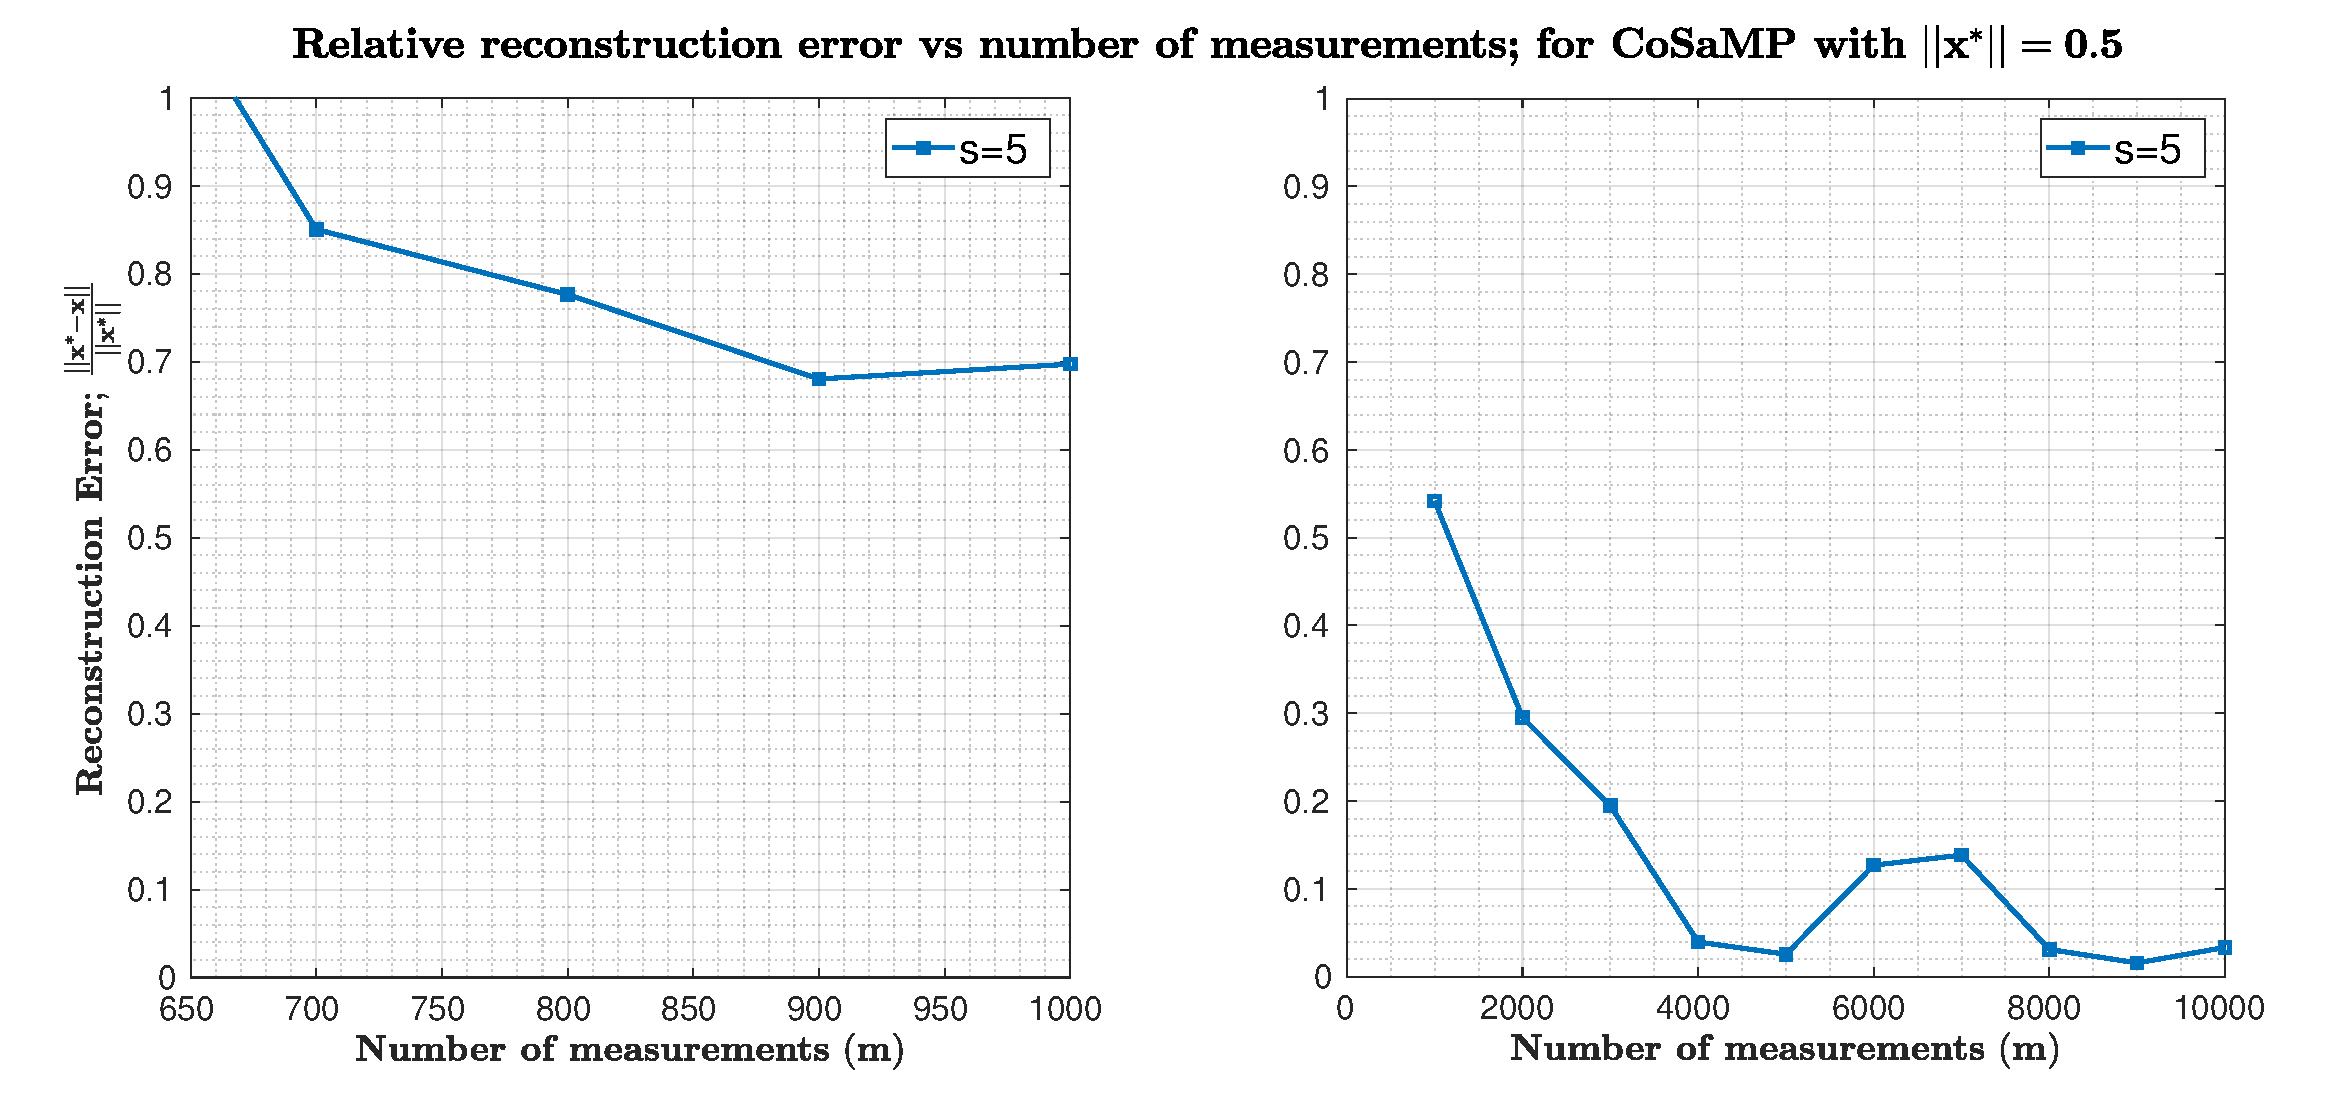
\includegraphics[width=\linewidth]{./fig/plot-1-2.pdf}
	\end{center}
	\caption{}
	\label{fig:plot-1-2}
\end{figure}
%
\begin{figure}[t]
	\begin{center}
		%\vspace{-0em}
		\includegraphics[width=\linewidth]{./fig/plot-1-3.pdf}
	\end{center}
	\caption{}
	\label{fig:plot-1-3}
\end{figure}
%
\begin{figure}[H]
	\begin{center}
		%\vspace{-0em}
		\includegraphics[width=\linewidth]{./fig/plot-1-1.pdf}
	\end{center}
	\caption{}
	\label{fig:plot-1-4}
\end{figure}
\section{Appendix}
\label{sec:append}
%\clearpage
%\input{../common/ack}
\bibliographystyle{plain}
\bibliography{./vsbib}
%\input{../common/appendix_a}
%\input{../common/appendix_b}

\end{document}